%File: anonymous-submission-latex-2023.tex
\documentclass[letterpaper]{article} % DO NOT CHANGE THIS
\usepackage{acl}
\usepackage{times}  % DO NOT CHANGE THIS
\usepackage{helvet}  % DO NOT CHANGE THIS
\usepackage{courier}  % DO NOT CHANGE THIS
\usepackage{graphicx} % DO NOT CHANGE THIS
\urlstyle{rm} % DO NOT CHANGE THIS
\def\UrlFont{\rm}  % DO NOT CHANGE THIS
\usepackage{natbib}  % DO NOT CHANGE THIS AND DO NOT ADD ANY OPTIONS TO IT
\usepackage{caption} % DO NOT CHANGE THIS AND DO NOT ADD ANY OPTIONS TO IT
\frenchspacing  % DO NOT CHANGE THIS
\setlength{\pdfpagewidth}{8.5in} % DO NOT CHANGE THIS
\setlength{\pdfpageheight}{11in} % DO NOT CHANGE THIS
%
% These are recommended to typeset algorithms but not required. See the subsubsection on algorithms. Remove them if you don't have algorithms in your paper.
\usepackage{algorithm}
\usepackage{algorithmic}
\usepackage{amsmath}
\usepackage{amssymb}
\usepackage{latexsym}
\usepackage{bbm}
\usepackage{multirow}
%
% These are are recommended to typeset listings but not required. See the subsubsection on listing. Remove this block if you don't have listings in your paper.
\usepackage{newfloat}
\usepackage{listings}
\DeclareCaptionStyle{ruled}{labelfont=normalfont,labelsep=colon,strut=off} % DO NOT CHANGE THIS
\lstset{%
	basicstyle={\footnotesize\ttfamily},% footnotesize acceptable for monospace
	numbers=left,numberstyle=\footnotesize,xleftmargin=2em,% show line numbers, remove this entire line if you don't want the numbers.
	aboveskip=0pt,belowskip=0pt,%
	showstringspaces=false,tabsize=2,breaklines=true}
\floatstyle{ruled}
\newfloat{listing}{tb}{lst}{}
\floatname{listing}{Listing}
%
% Keep the \pdfinfo as shown here. There's no need
% for you to add the /Title and /Author tags.
\pdfinfo{
/TemplateVersion (2023.1)
}

% DISALLOWED PACKAGES
% \usepackage{authblk} -- This package is specifically forbidden
% \usepackage{balance} -- This package is specifically forbidden
% \usepackage{color (if used in text)
% \usepackage{CJK} -- This package is specifically forbidden
% \usepackage{float} -- This package is specifically forbidden
% \usepackage{flushend} -- This package is specifically forbidden
% \usepackage{fontenc} -- This package is specifically forbidden
% \usepackage{fullpage} -- This package is specifically forbidden
% \usepackage{geometry} -- This package is specifically forbidden
% \usepackage{grffile} -- This package is specifically forbidden
% \usepackage{hyperref} -- This package is specifically forbidden
% \usepackage{navigator} -- This package is specifically forbidden
% (or any other package that embeds links such as navigator or hyperref)
% \indentfirst} -- This package is specifically forbidden
% \layout} -- This package is specifically forbidden
% \multicol} -- This package is specifically forbidden
% \nameref} -- This package is specifically forbidden
% \usepackage{savetrees} -- This package is specifically forbidden
% \usepackage{setspace} -- This package is specifically forbidden
% \usepackage{stfloats} -- This package is specifically forbidden
% \usepackage{tabu} -- This package is specifically forbidden
% \usepackage{titlesec} -- This package is specifically forbidden
% \usepackage{tocbibind} -- This package is specifically forbidden
% \usepackage{ulem} -- This package is specifically forbidden
% \usepackage{wrapfig} -- This package is specifically forbidden
% DISALLOWED COMMANDS
% \nocopyright -- Your paper will not be published if you use this command
% \addtolength -- This command may not be used
% \balance -- This command may not be used
% \baselinestretch -- Your paper will not be published if you use this command
% \clearpage -- No page breaks of any kind may be used for the final version of your paper
% \columnsep -- This command may not be used
% \newpage -- No page breaks of any kind may be used for the final version of your paper
% \pagebreak -- No page breaks of any kind may be used for the final version of your paperr
% \pagestyle -- This command may not be used
% \tiny -- This is not an acceptable font size.
% \vspace{- -- No negative value may be used in proximity of a caption, figure, table, section, subsection, subsubsection, or reference
% \vskip{- -- No negative value may be used to alter spacing above or below a caption, figure, table, section, subsection, subsubsection, or reference

\setcounter{secnumdepth}{0} %May be changed to 1 or 2 if section numbers are desired.

% The file aaai23.sty is the style file for AAAI Press
% proceedings, working notes, and technical reports.
%

% Title

% Your title must be in mixed case, not sentence case.
% That means all verbs (including short verbs like be, is, using,and go),
% nouns, adverbs, adjectives should be capitalized, including both words in hyphenated terms, while
% articles, conjunctions, and prepositions are lower case unless they
% directly follow a colon or long dash
\title{Supplementary Material for Knowledge Graph Reasoning with Self-supervised Reinforcement Learning}


% REMOVE THIS: bibentry
% This is only needed to show inline citations in the guidelines document. You should not need it and can safely delete it.
\usepackage{bibentry}
% END REMOVE bibentry

\begin{document}
\maketitle

\appendix
\begin{figure*}[h!] 
    \centering
    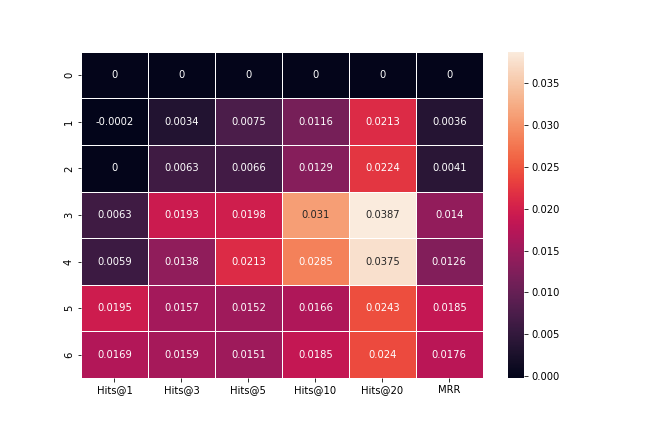
\includegraphics[scale=0.4]{fig/fb15k-237_minerva_zeroed_heatmap.png}\hspace{-15mm}
    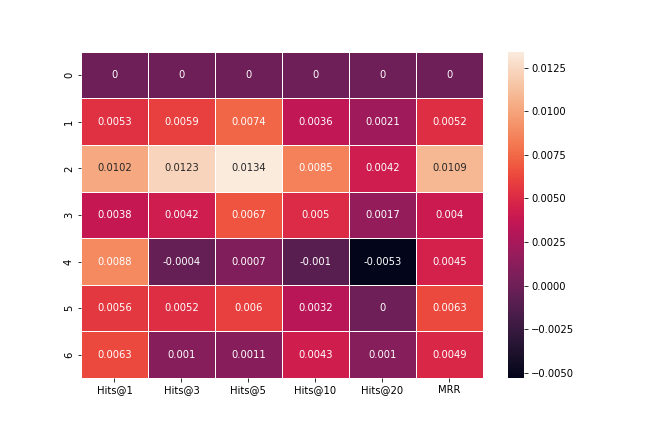
\includegraphics[scale=0.4]{fig/wn18rr_minerva_zeroed_heatmap.png}\hspace{-15mm}\\
    (a) FB15K-237  \hspace{50mm}  (b) WN18RR\\
    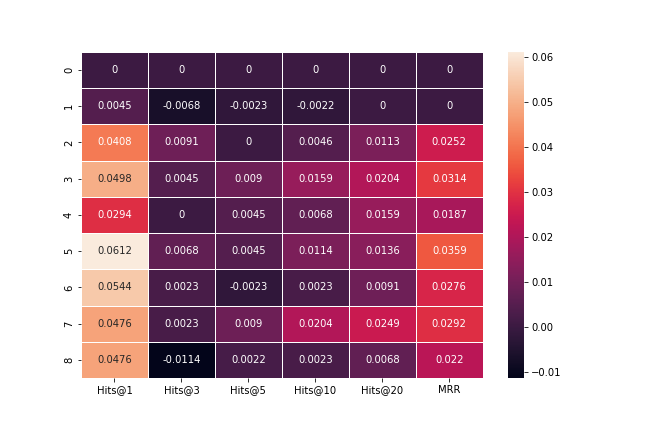
\includegraphics[scale=0.4]{fig/nell995_minerva_zeroed_heatmap.png}\hspace{-15mm}
    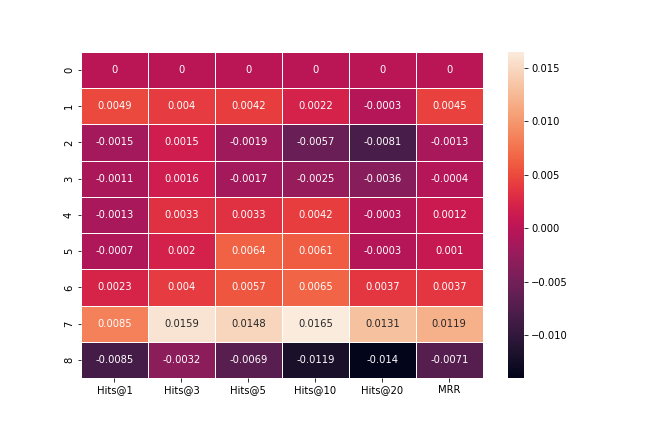
\includegraphics[scale=0.4]{fig/fb60k-nyt10_minerva_zeroed_heatmap.png}\\
    (c) NELL-995 \hspace{50mm} (d) FB60K
    \caption{Heatmap of Hits@k and MRR metrics for different SL training epochs followed by RL training. MINERVA is the baseline (SS-MINERVA) here. Row 0 is pure RL. The value in each cell is the score for that cell minus the score for that category at epoch 0 to highlight the difference.}
    \label{fig:heatmap_all}
\end{figure*}
\section{Appendix 1 Hyperparameter}

\paragraph{RL agent} The hyperparameters related to the RL part of our SS-MINERVA and SS-MultihopKG are the same as the original paper for FB15K-237, NELL-995 and WN18RR. 

Since this is the first work applying MINERVA to FB60K, we tried our best to adjust the hyperparameters to achieve the best performance. The size of the network is the same as FB15K-237. We also use the Wavier initialization for the embedding and neural network. The weight parameter $\beta$ for the entropy regularization term is 0.02 and the learning rate is $1^{-3}$. 


\paragraph{SL agent} We keep all the hyperparamters for SL agent such as the the number of layers, the number of neurons in each layer, the paramters of LSTM the same as the RL agent. The learning rate for the SL agent is $1^{-3}$. 





\section{Appendix 2 Performance analysis}
\label{sec:appendix}
In Fig. \ref{fig:heatmap_all}, we show the heatmaps of Hits@k and MRR metrics for all four datasets (we only show the heatmaps of FB15K-237 and FB60K in the main manuscript). From the results, we can see that the agent achieves its best performance with three, two, five, and seven epochs of SL pretraining on FB1K-237, WN18RR, NELL-995 and FB60K respectively. The results reported in Table 2 and 3 are based on these SL training epochs. 



From Table 2 and Table 3 in the main manuscript, we can see that the improvements of SSRL to RL on different KG datsets are quite different. The improvements on FB15K-237 and NELL-995 datasets are significant. However, the improvement on WN18RR is mediocre and FB60K is moderate. We think there are two reasons for it: 
\begin{itemize}
    \item The imbalanced training data for different relation types.
    \item The small graph degree (number of edges connecting to each edge);
\end{itemize}


In order to verify this two assumptions, we show the distribution of relations in the training set in Fig.\ref{fig:relation distribtion}. On NELL, which the agent performs the best on out of all the datasets, there are an even distribution of relation types that show up with different frequencies in the dataset. This means that the agent is seeing a good sample of the different query types, and trains well on all of them. On WN18RR and FB60K, the distributions of relation types are very skewed. 

For WN18RR, where the improvement of SSRL on RL is most insignificant, just two relations types comprise more than 75\% of the dataset while the others show up comparatively infrequently. Since the goal of SL is to learn the underlying distribution based on labeled data and in doing encourage the agent to explore paths it wouldn't otherwise, pretraining on these skewed distributions would encourage the agent to find more correct paths on the dominate relations, so it achieves higher overall accuracy on the whole training set. However, it may sacrifice the performance on less common relations where finding even one correct path is difficult. Furthermore, the idea behind SL is that by teaching the agent this underlying distribution it may take potentially advantageous paths it otherwise wouldn't take; if the the dataset is nostly homogenous (e.g. sharply skewed towards a select few relations), there is little that SL could show the agent that it wouldn't find during RL anywways. As the a result, SL pretraining does not help in terms of Hits@k when k is large on sharply skewed datasets like WN18RR 

For FB60K, Fig.\ref{fig:heatmap_all} shows that the trial where a correct path was found for the highest percentage of queries uses 7000 steps of SL. The graphs in Fig.\ref{fig:learing curve} in the main manuscript track average reward over the batch, which includes multiple trials for each query. Our analysis of agent performance by relation type included in Fig.\ref{fig:relation distribtion} shows that FB60K is the only dataset containing numerous relations with a near 100\% fact prediction success rate, implying that it contains facts easier for the agent to understand. Intuitively, the immediately strong performance on these "low hanging fruit" will increase the average performance towards the beginning of training, but as increasing durations of SL pretraining force the agent to generalize to more complex relations its success rate on these relations naturally falls, resulting in a decreasing average performance and an increasing percentage of queries for which a correct path is found. This tracks with the graph and heatmap presented in Fig.\ref{fig:learing curve} in the main manuscript and Fig.\ref{fig:heatmap_all}.

To backup these claim, we plot the learning curves with Hit@20 as the metric in Fig.\ref{fig:learing curve2}. The SL graphs show negative trends on skewed datasets, i.e., WN18RR and FB60K. This is reasonable because the target of SL is to minimize the crossentropy loss, therefore maximize the overall accuracy. It is noted that the final performance on Hits@20 can be fixed by the RL training stage. This also shows to importance of the RL training stage in the proposed architecture.

We also observed that our SSRL architecture performs very well on FB15K-237 where the relation type distribution is also skewed (although it is less skewed than FB60K and WN18RR). We believe the excellent performance is due to the high graph degree where the SL are particularly helpful. Table 1 of the main manuscript shows the median degree of FB15K-237 is 14 whereas other datasets is less than 4.

In summary, the extent of improvement of SSRL to RL depends on the statistics of the datasets such as graph degree and relation distributions. Currently, our SSRL architecture generates labels for random relation types. In our future work, we will discuss how to generate labels based on the relation disctributions in each dataset therefore improve the performance further.

\begin{figure*}
    \centering
    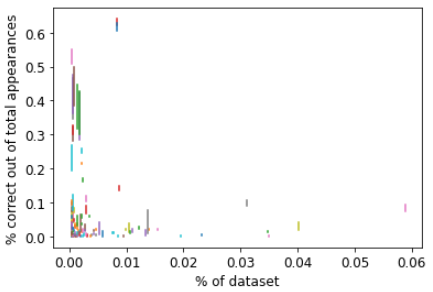
\includegraphics[scale=0.6]{fig/FB15K_acc_increase.png}
    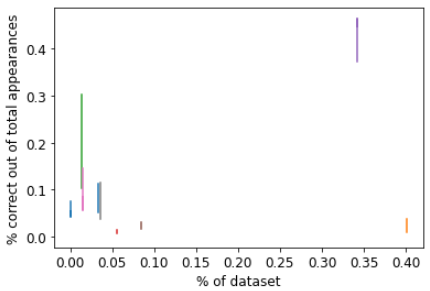
\includegraphics[scale=0.6]{fig/WN18RR_acc_increase.png}\\
    (a) FB15K-237  \hspace{50mm}  (b) WN18RR\\
    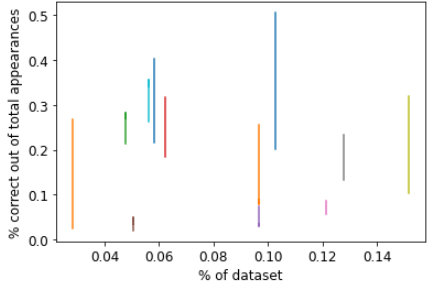
\includegraphics[scale=0.6]{fig/NELL_acc_increase.png}
    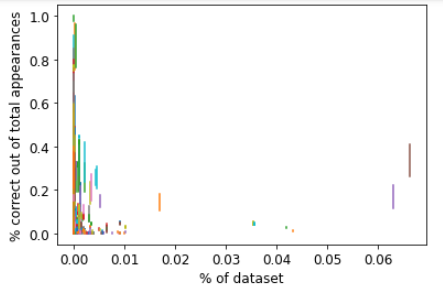
\includegraphics[scale=0.6]{fig/FB60K_acc_increase.png}\\
    (c) NELL-995 \hspace{50mm} (d) FB60K
    \caption{Distribution of relations in the training set. The vertical lines correspond to the accuracy of the agent on that relation increasing over the course of training}
    \label{fig:relation distribtion}
\end{figure*}









\begin{figure*}[h] 
    \centering
    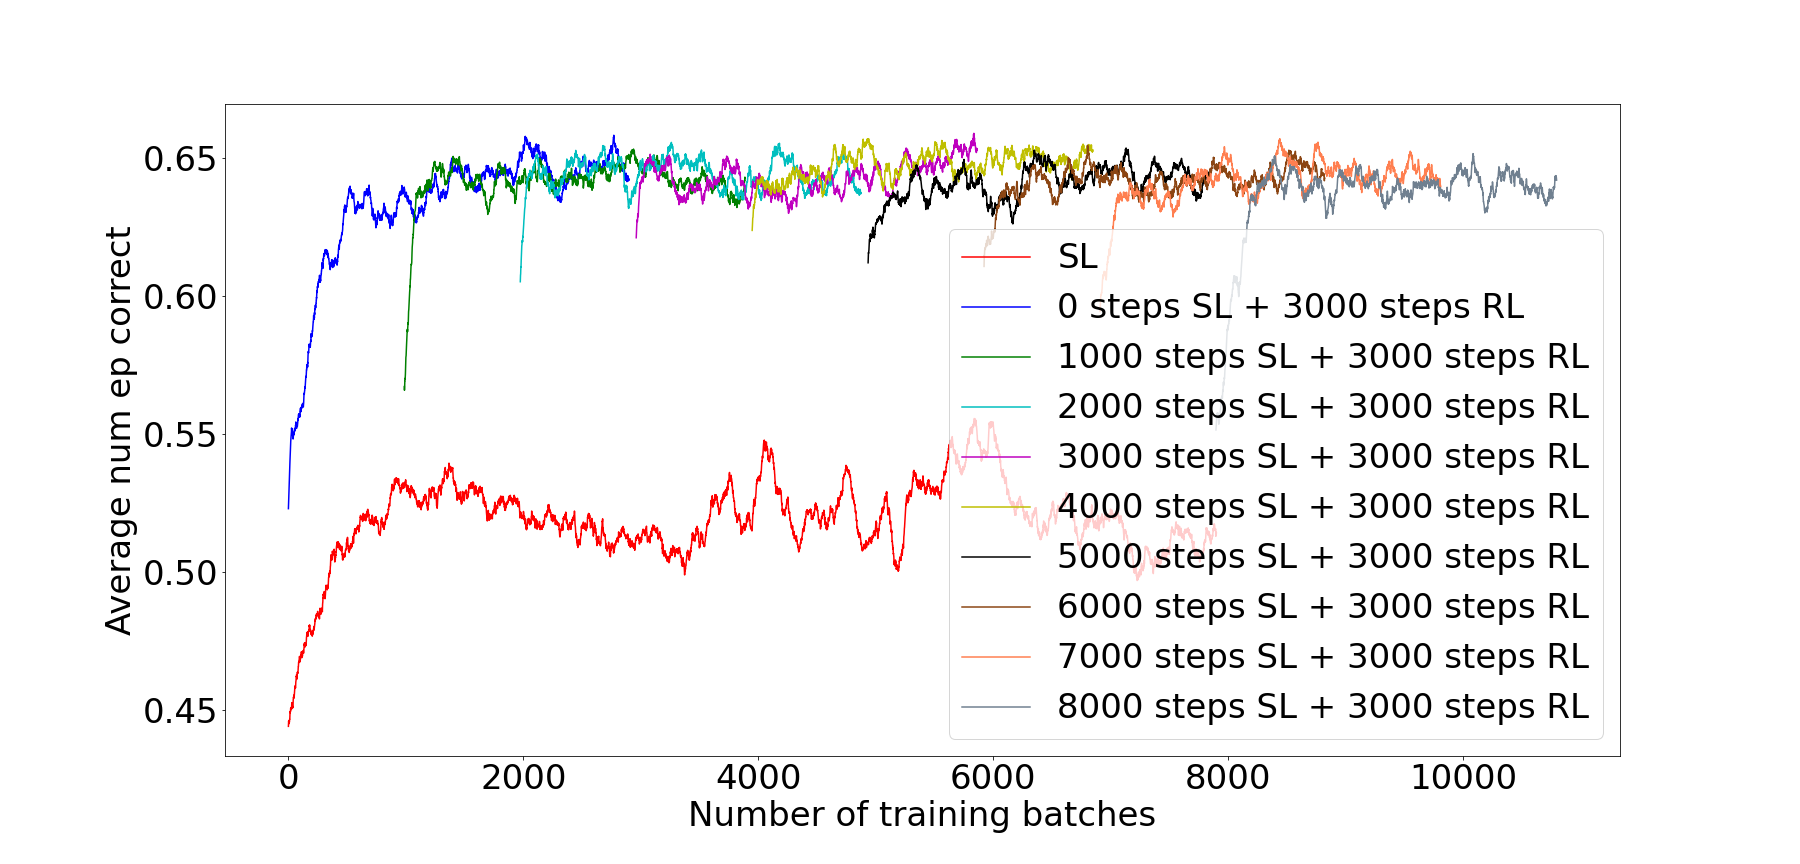
\includegraphics[scale=0.14]{fig/FB15K_correct.png}\hspace{-10mm} 
    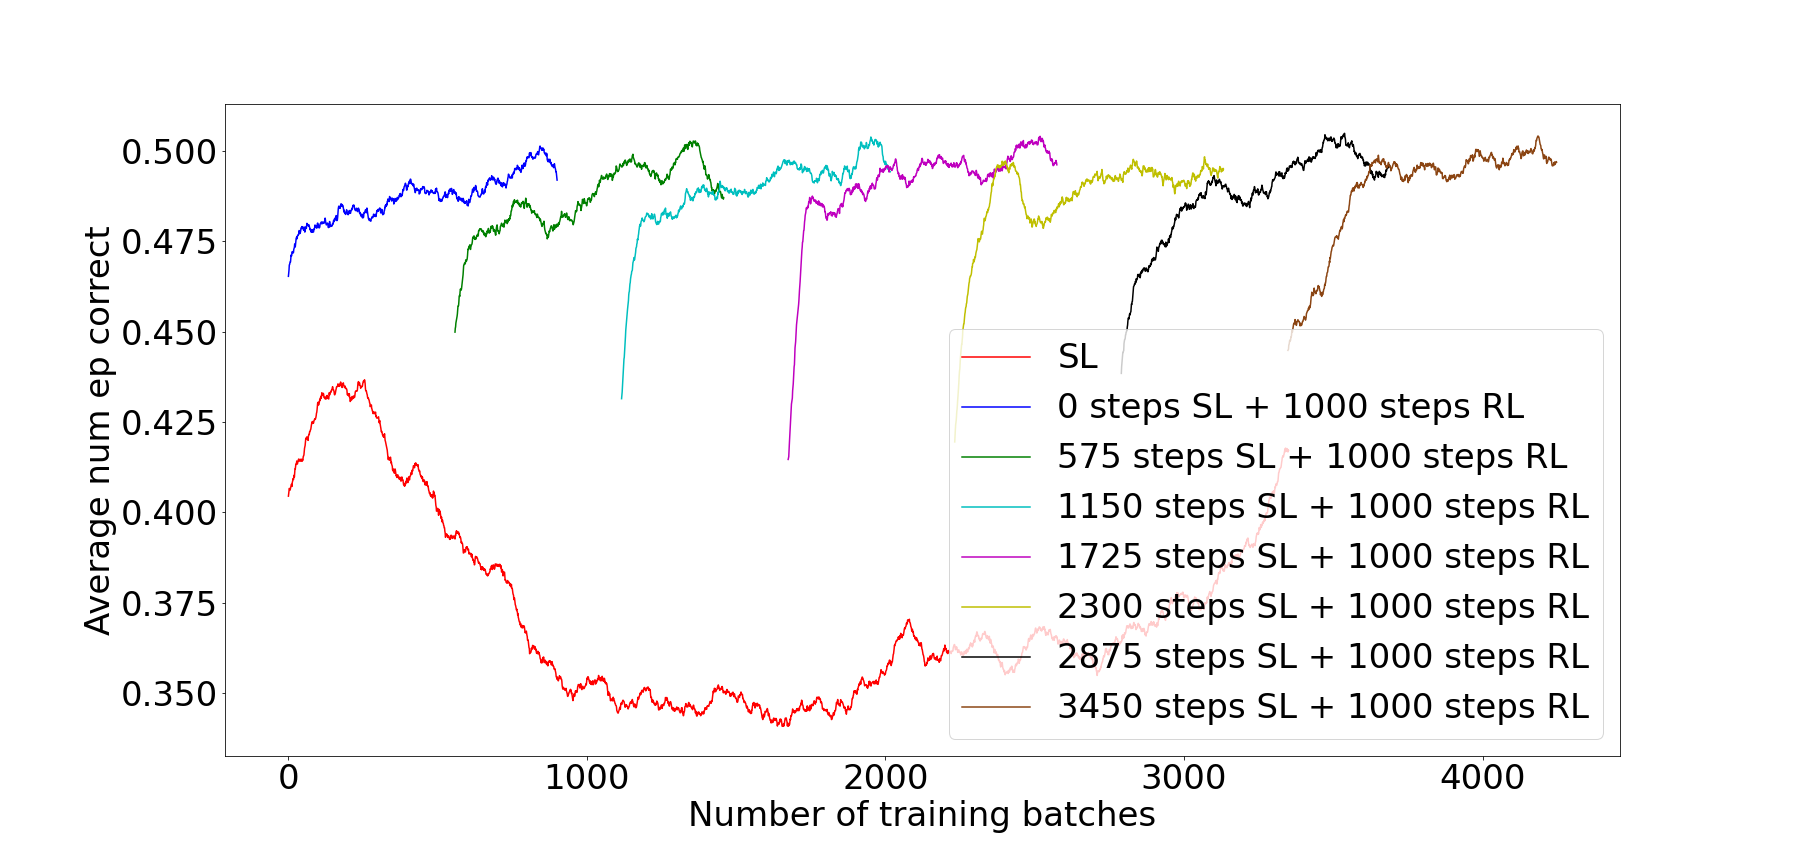
\includegraphics[scale=0.14]{fig/WN18RR_correct.png}\\
    (a) FB15K-237  \hspace{45mm}  (b) WN18RR\\
    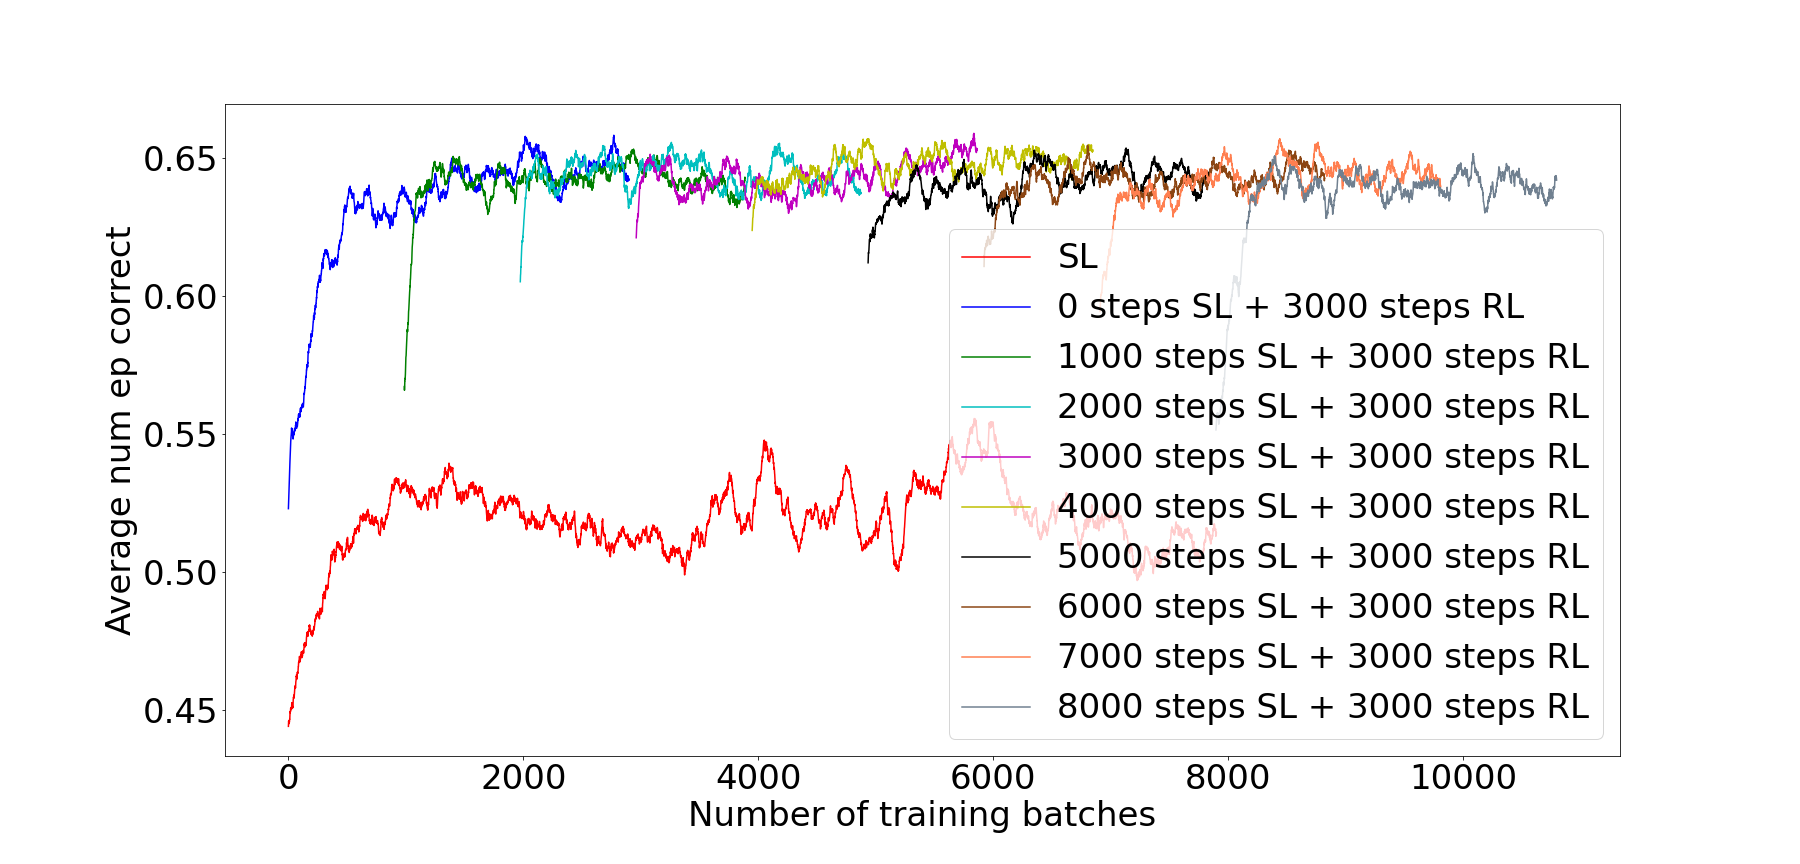
\includegraphics[scale=0.14]{fig/NELL_correct.png}\hspace{-10mm} 
    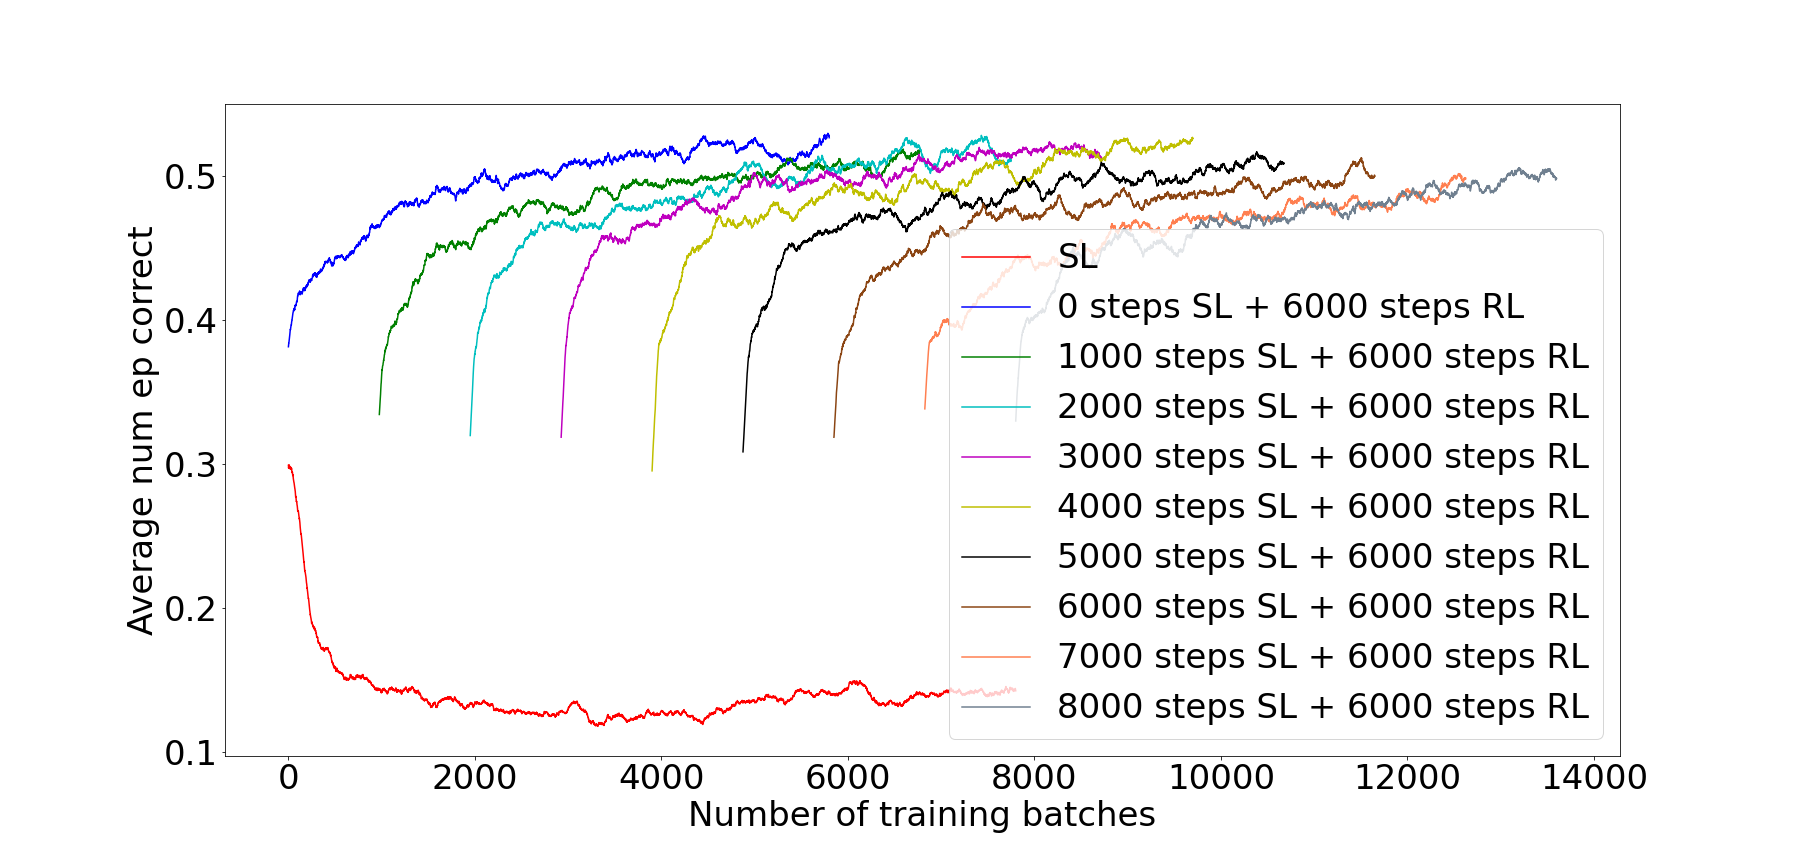
\includegraphics[scale=0.14]{fig/FB60K_correct.png}\\
    (c) NELL-995 \hspace{45mm} (d) FB60K
    \caption{Learning curves ((Hits@20 v.s. number of training batches)) with different SL pretraining steps followed by same RL steps}
    \label{fig:learing curve2}
\end{figure*}







\end{document}


\begin{table*}
\centering
\begin{tabular}{llccc}
\hline
\textbf{Data} & Metric& M-Walk reproduced& MINERVA & Our reproduced  \\
\multirow{4}{4em}{FB15K-237} & HITS@1& 14.1& 21.7&-\\
& HITS@3 & 23.2&32.9&-\\
& HITS@10 &-&45.6&-\\
& MRR &20.5&29.3&-\\
\hline
\multirow{4}{4em}{WN18RR} & HITS@1&35.1&41.3&45\\
& HITS@3 &44.5&45.6&49\\
& HITS@10 &-&51.3&55\\
& MRR &40.9&44.8&48\\
\hline
\multirow{4}{4em}{NELL-995} & HITS@1&-&66.3&65\\
& HITS@3 &-&77.3&80\\
& HITS@10 &- &83.1 &82\\
& MRR &- &72.5&73\\
\hline
\end{tabular}
\caption{Statistics of datasets used in experiments
}
\label{dataset}
\end{table*}

\begin{figure*} 
    \centering
    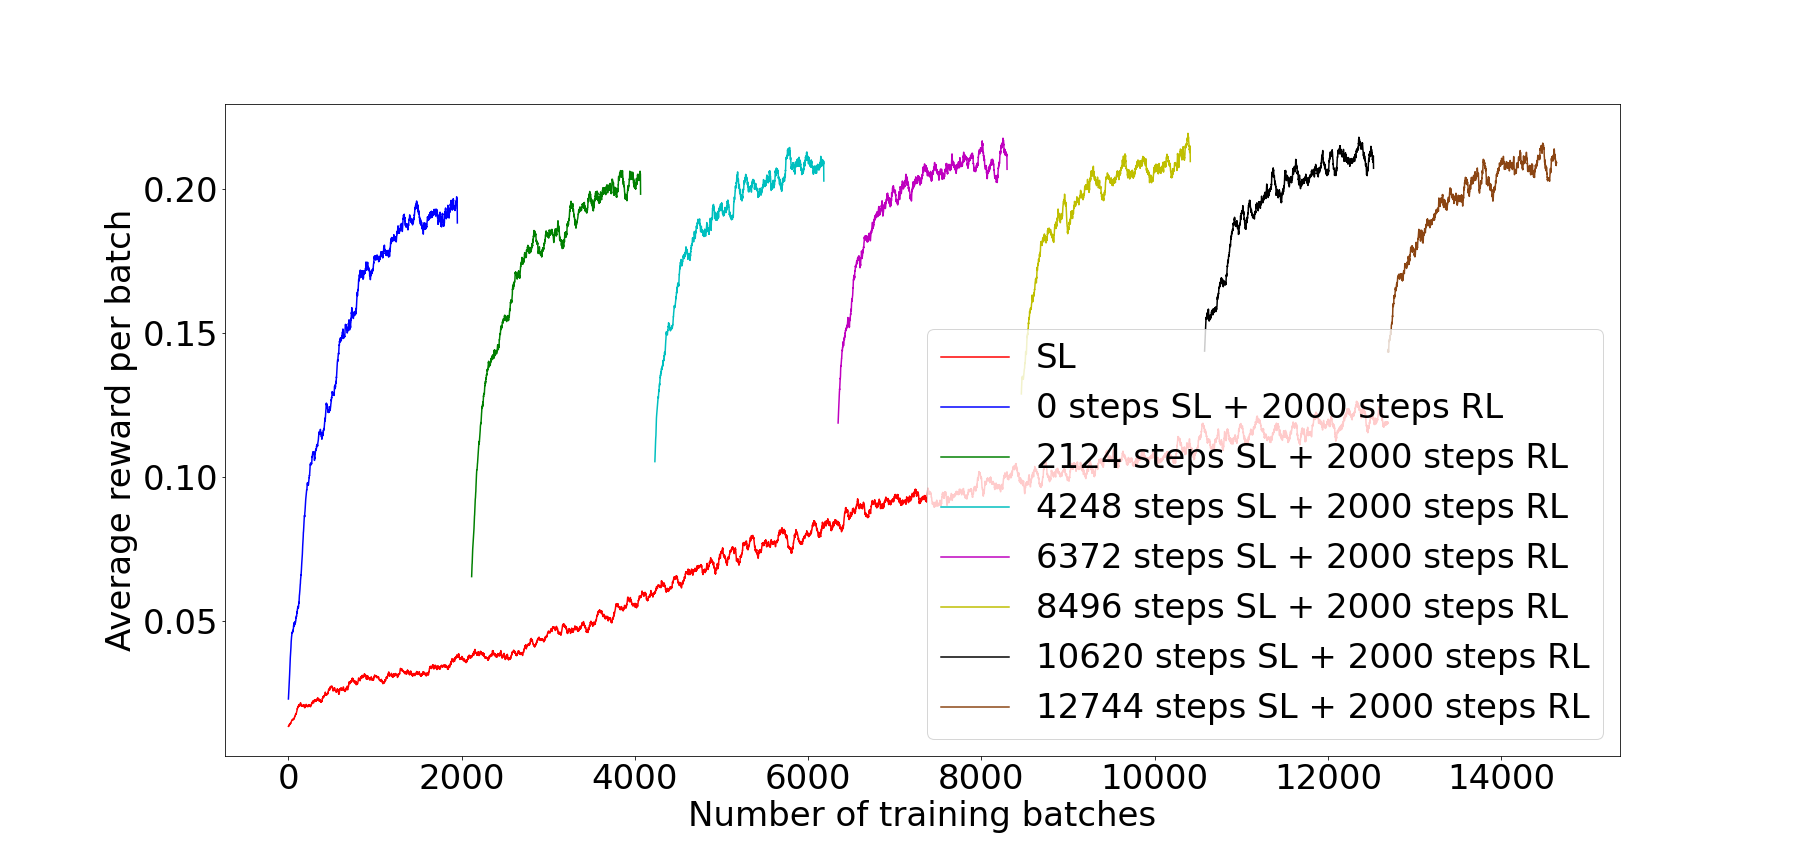
\includegraphics[scale=0.55]{fig/FB15K_acc.png}
    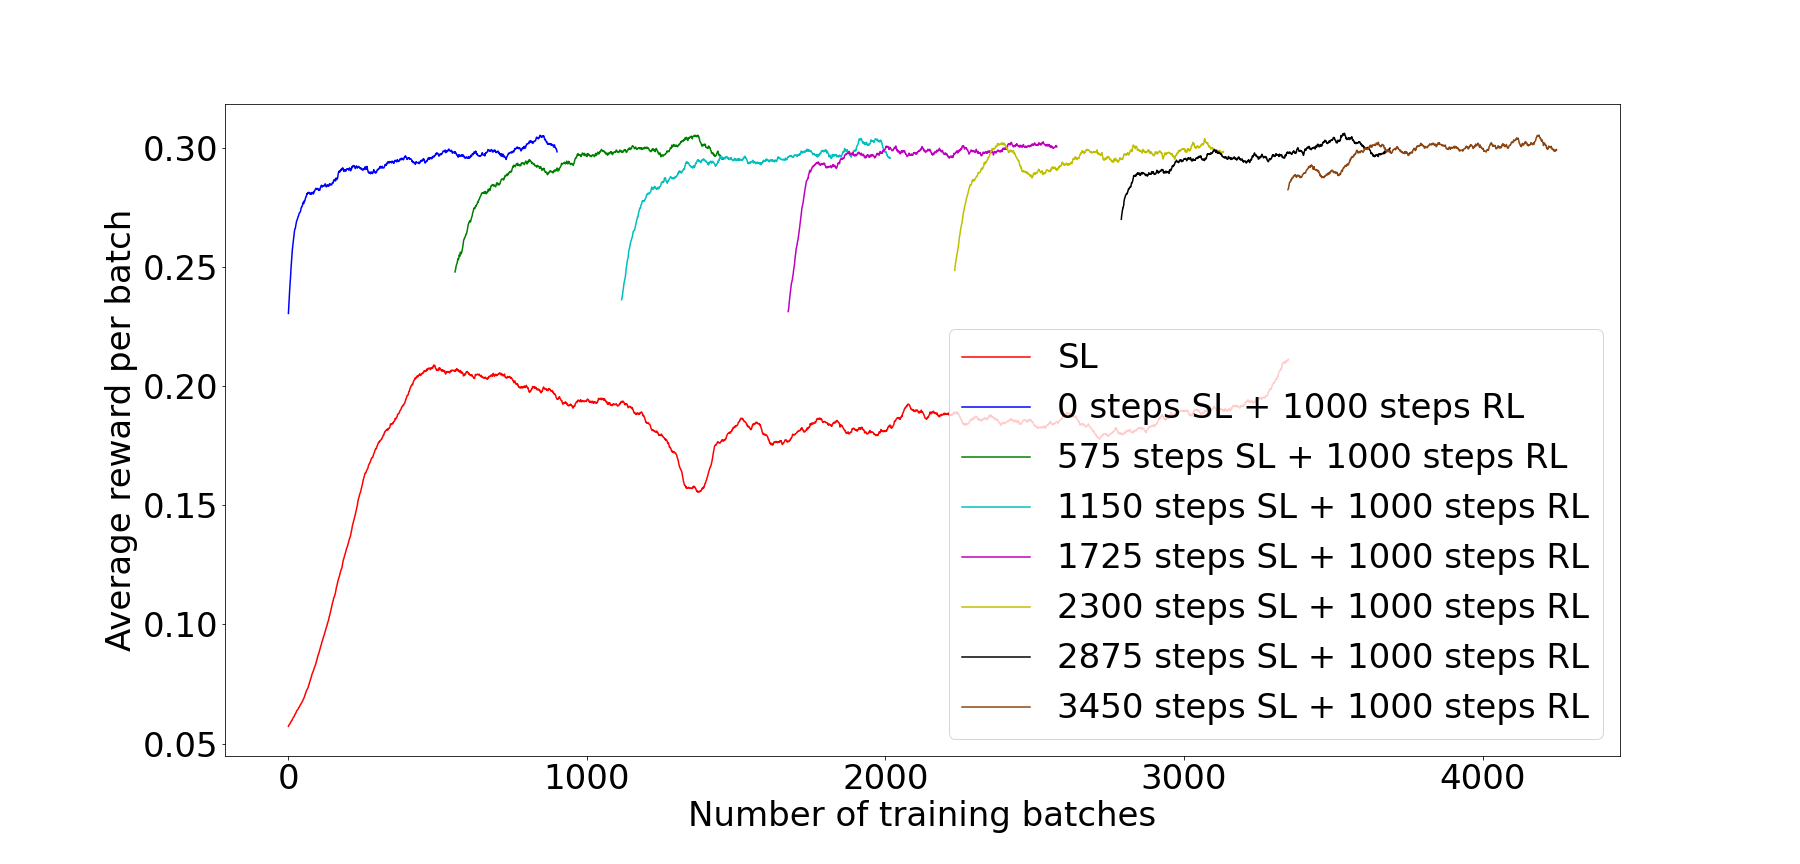
\includegraphics[scale=0.55]{fig/WN18RR_acc.png}\hspace{-15mm}\\
    (a) FB15K-237  \hspace{45mm}  (b) WN18RR\\
    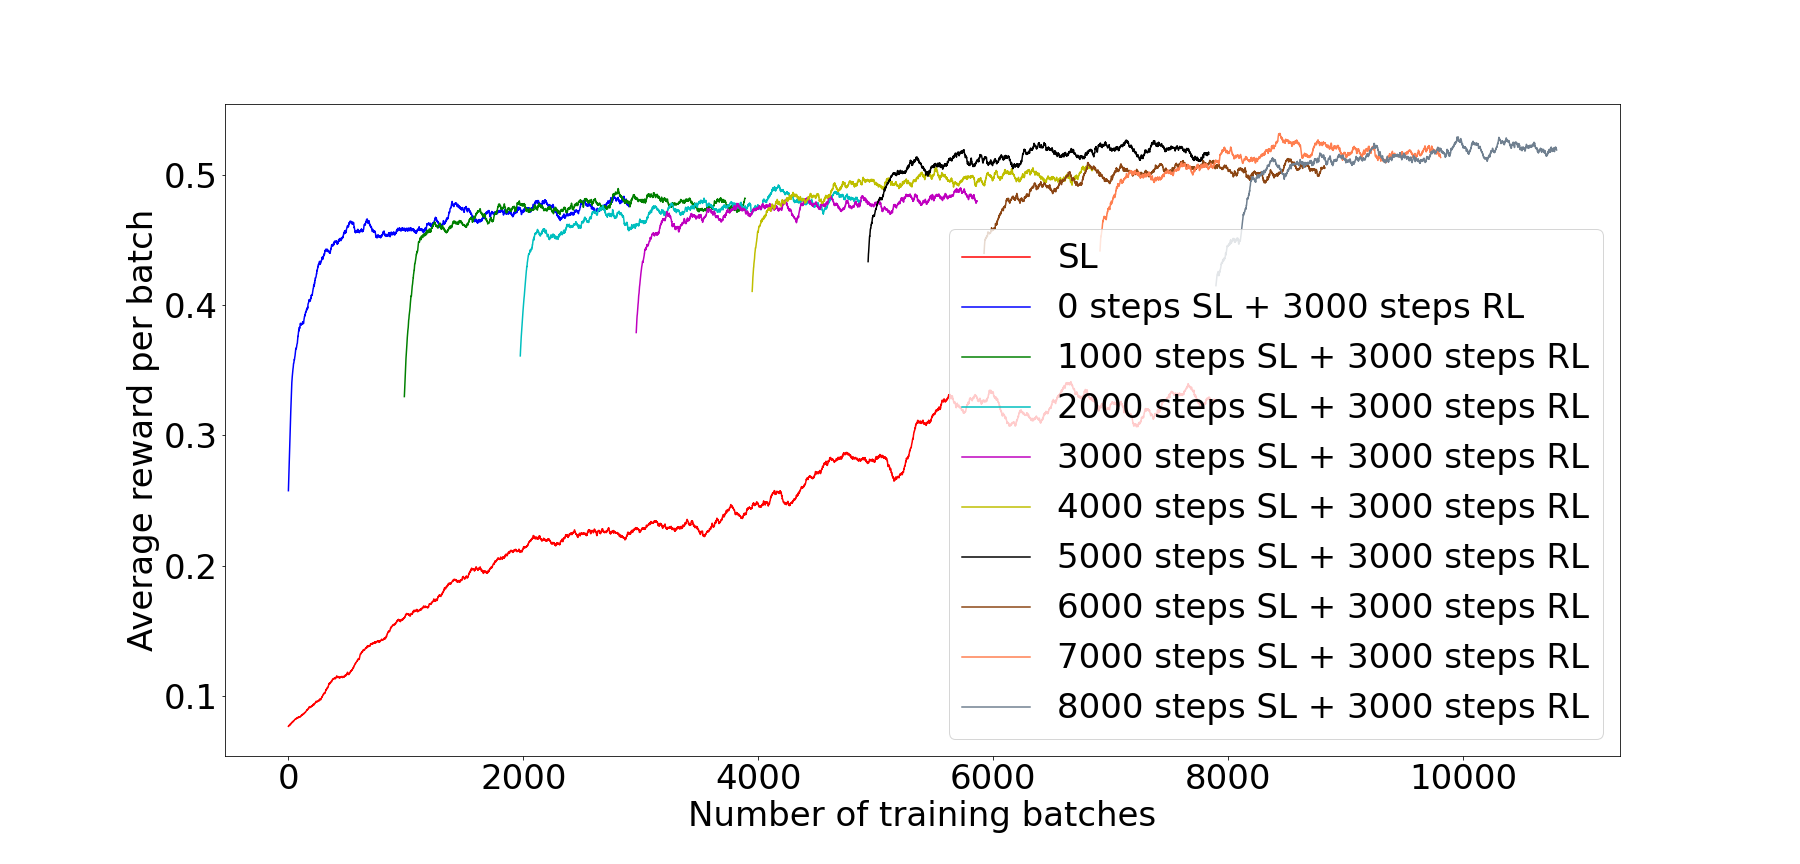
\includegraphics[scale=0.55]{fig/NELL_acc.png}
    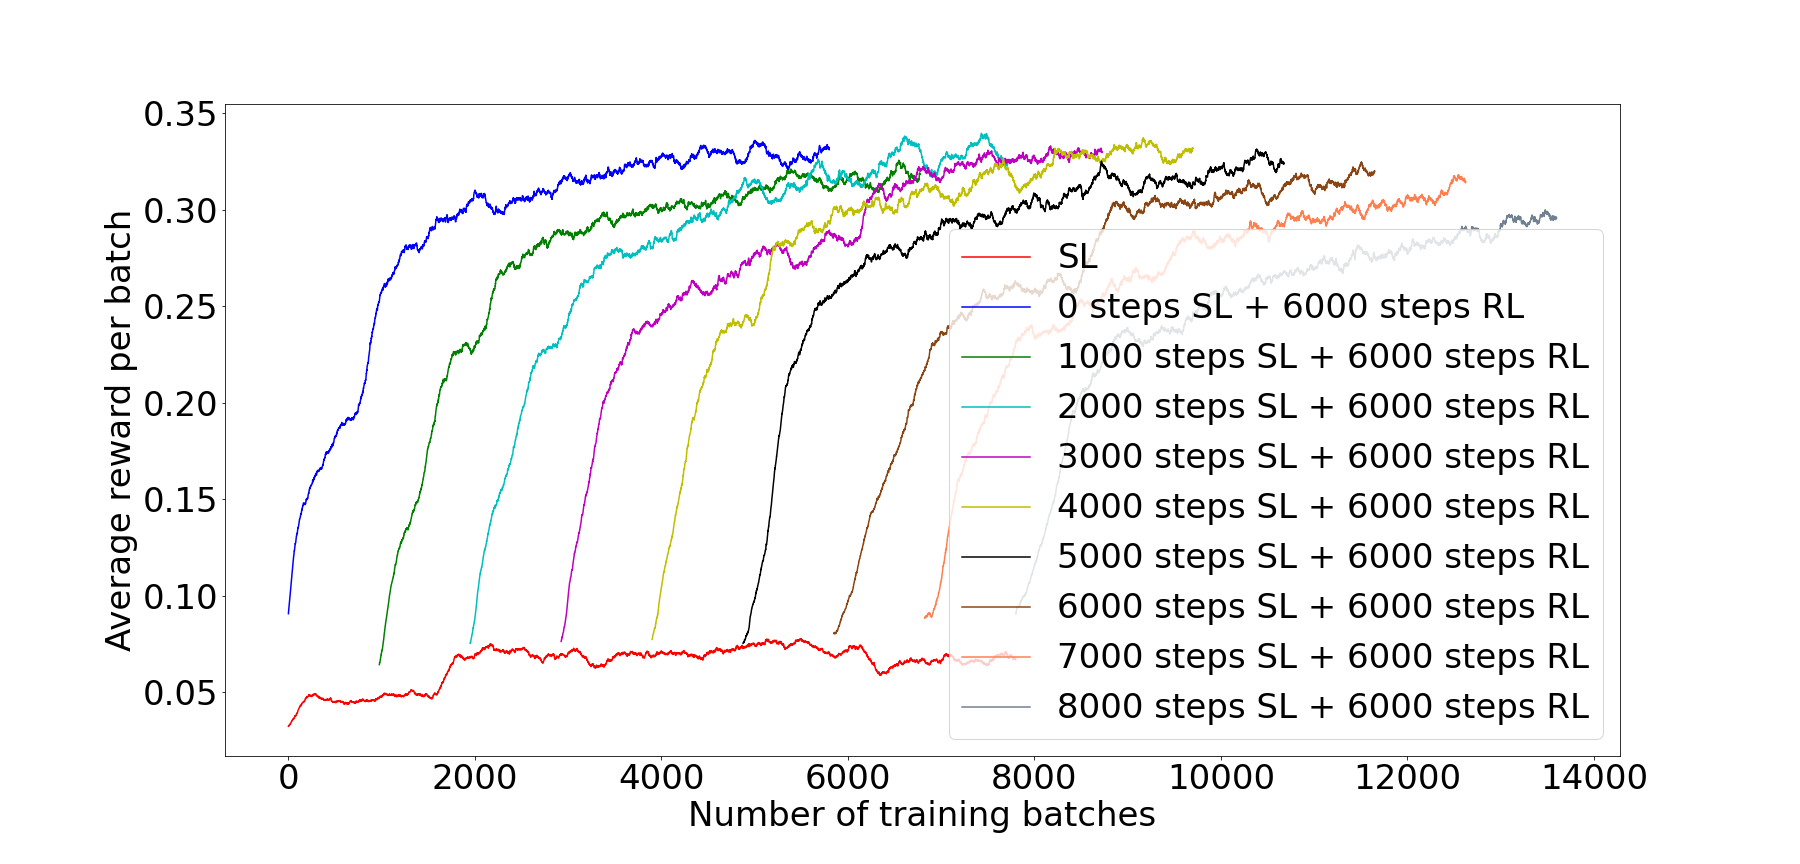
\includegraphics[scale=0.55]{fig/FB60K_acc.png}\\
    (c) NELL-995 \hspace{45mm} (d) FB60K
    \caption{Caption}
    \label{fig:heatmap}
\end{figure*}
\begin{table}
\centering
\begin{tabular}{lllll}
\hline
\multicolumn{2}{c}{\textbf{Answer Range}} & \textbf{RL} & \textbf{SL}& \textbf{SSRL}\\
\hline
\multirow{2}{4em}{1hop} & Hits@1 &1 &2 &3 \\
 &Hits@3 & & &  \\
 &Hits@10 & & & \\
 \hline
\multirow{2}{4em}{2hops} & Hits@1 &1 &2 &3 \\
 &Hits@3 & & &  \\
 &Hits@10 & & & \\
 \hline
 \multirow{2}{4em}{3hops} & Hits@1 &1 &2 &3 \\
 &Hits@3 & & &  \\
 &Hits@10 & & & \\
\hline
\end{tabular}
\caption{performance on different answer distribution}
\end{table}


\begin{table}
\centering
\begin{tabular}{lllll}
\hline
\multicolumn{2}{c}{\textbf{\# Existing Paths}} & \textbf{RL} & \textbf{SL}& \textbf{SSRL}\\
\hline
\multirow{2}{4em}{0-50} & Hits@1 &1 &2 &3 \\
 &Hits@3 & & &  \\
 &Hits@10 & & & \\
 \hline
\multirow{2}{4em}{50-100} & Hits@1 &1 &2 &3 \\
 &Hits@3 & & &  \\
 &Hits@10 & & & \\
 \hline
 \multirow{2}{4em}{100-200} & Hits@1 &1 &2 &3 \\
 &Hits@3 & & &  \\
 &Hits@10 & & & \\
  \multirow{2}{4em}{200-500} & Hits@1 &1 &2 &3 \\
 &Hits@3 & & &  \\
 &Hits@10 & & & \\
  \multirow{2}{4em}{500-} & Hits@1 &1 &2 &3 \\
 &Hits@3 & & &  \\
 &Hits@10 & & & \\
\hline
\end{tabular}
\caption{performance on different number of correct paths}
\end{table}

\begin{table}
\centering
\begin{tabular}{lllll}
\hline
\multicolumn{2}{c}{\textbf{Answer Range}} & \textbf{RL} & \textbf{SL}& \textbf{SSRL}\\
\hline
\multirow{2}{4em}{to one} & Hits@1 &1 &2 &3 \\
 &Hits@3 & & &  \\
 &Hits@10 & & & \\
 \hline
\multirow{2}{4em}{to many} & Hits@1 &1 &2 &3 \\
 &Hits@3 & & &  \\
 &Hits@10 & & & \\
\hline
\end{tabular}
\caption{performance on different answer distribution}
\end{table}

We also evaluate the effectiveness of the supervised pretraining with partial labels on a large KG dataset (FB60k) when generating labels for all training queries is infeasible.
This is a section in the appendix.

\begin{figure}[h!] 
    \centering
    \includegraphics[scale=0.3]{fig/combine distribution.png}
    \caption{Caption}
    \label{fig:sys}
\end{figure}